
%(BEGIN_QUESTION)
% Copyright 2006, Tony R. Kuphaldt, released under the Creative Commons Attribution License (v 1.0)
% This means you may do almost anything with this work of mine, so long as you give me proper credit

Calculate values for the following calibration table, for a displacer-type level transmitter measuring liquid level interface (specific gravities = 0.9 and 2.0), with a calibration tolerance of $\pm$ 1\%:

$$\includegraphics[width=15.5cm]{i00314x01.eps}$$

% No blank lines allowed between lines of an \halign structure!
% I use comments (%) instead, so that TeX doesn't choke.

$$\vbox{\offinterlineskip
\halign{\strut
\vrule \quad\hfil # \ \hfil & 
\vrule \quad\hfil # \ \hfil & 
\vrule \quad\hfil # \ \hfil & 
\vrule \quad\hfil # \ \hfil & 
\vrule \quad\hfil # \ \hfil & 
\vrule \quad\hfil # \ \hfil \vrule \cr
\noalign{\hrule}
%
% First row
Interface & Percent of & Buoyant & Output signal & Output signal & Output signal \cr
%
% Another row
level (in) & span (\%) & force (lbs) & ideal (PSI) & min. (PSI) & max. (PSI) \cr
%
\noalign{\hrule}
%
% Another row
  & 0 &  &  &  &  \cr
%
\noalign{\hrule}
%
% Another row
  & 10 &  &  &  &  \cr
%
\noalign{\hrule}
%
% Another row
  & 25 &  &  &  &  \cr
%
\noalign{\hrule}
%
% Another row
  & 50 &  &  &  &  \cr
%
\noalign{\hrule}
%
% Another row
  & 75 &  &  &  &  \cr
%
\noalign{\hrule}
%
% Another row
  & 90 &  &  &  &  \cr
%
\noalign{\hrule}
%
% Another row
  & 100 &  &  &  &  \cr
%
\noalign{\hrule}
} % End of \halign 
}$$ % End of \vbox

Assume the following displacer characteristics:

\begin{itemize}
\item{} Shape: {\it cylindrical}
\item{} Length = 15 inches
\item{} Diameter = 2 inches
\item{} Dry weight = 4.5 lbs
\end{itemize}

\vskip 10pt

Be sure to show all your mathematical work so that your instructor will be able to check the conceptual validity of your technique(s).  A good way to check to see if you're solving the problem correctly is to check that each and every one of your intermediate calculations (i.e. the results you get mid-way during the process to arrive at the final answer) has real physical meaning.  {\bf If you truly understand what you are doing, you will be able to identify the correct unit of measurement for every intermediate result and also be able to show where that number applies to the scenario at hand}.


\vskip 20pt \vbox{\hrule \hbox{\strut \vrule{} {\bf Suggestions for Socratic discussion} \vrule} \hrule}

\begin{itemize}
\item{} Two technicians are arguing about the operation of a displacer-type level transmitter.  One thinks that static pressure inside the process vessel affects accuracy, while the other technician thinks it doesn't.  Who is correct, and why?
\item{} Demonstrate how to {\it estimate} numerical answers for this problem without using a calculator.
\end{itemize}

\underbar{file i00314}
%(END_QUESTION)





%(BEGIN_ANSWER)

\noindent
{\bf Partial answer:}

% No blank lines allowed between lines of an \halign structure!
% I use comments (%) instead, so that TeX doesn't choke.

$$\vbox{\offinterlineskip
\halign{\strut
\vrule \quad\hfil # \ \hfil & 
\vrule \quad\hfil # \ \hfil & 
\vrule \quad\hfil # \ \hfil & 
\vrule \quad\hfil # \ \hfil & 
\vrule \quad\hfil # \ \hfil & 
\vrule \quad\hfil # \ \hfil \vrule \cr
\noalign{\hrule}
%
% First row
Interface & Percent of & Buoyant & Output signal & Output signal & Output signal \cr
%
% Another row
level (in) & span (\%) & force (lbs) & ideal (PSI) & min. (PSI) & max. (PSI) \cr
%
\noalign{\hrule}
%
% Another row
0 & 0 &  &  &  & 3.12 \cr
%
\noalign{\hrule}
%
% Another row
 & 10 &  &  & 4.08 &  \cr
%
\noalign{\hrule}
%
% Another row
 & 25 &  &  &  &  \cr
%
\noalign{\hrule}
%
% Another row
 & 50 & 2.469 &  &  &  \cr
%
\noalign{\hrule}
%
% Another row
11.25 & 75 &  &  &  &  \cr
%
\noalign{\hrule}
%
% Another row
 & 90 &  &  &  &  \cr
%
\noalign{\hrule}
%
% Another row
 & 100 &  & 15 &  &  \cr
%
\noalign{\hrule}
} % End of \halign 
}$$ % End of \vbox

%(END_ANSWER)





%(BEGIN_NOTES)

Here are the two ``thought experiment'' scenarios pictured to arrive at the LRV and URV pressure values:

$$\includegraphics[width=15.5cm]{i00314x02.eps}$$

% No blank lines allowed between lines of an \halign structure!
% I use comments (%) instead, so that TeX doesn't choke.

$$\vbox{\offinterlineskip
\halign{\strut
\vrule \quad\hfil # \ \hfil & 
\vrule \quad\hfil # \ \hfil & 
\vrule \quad\hfil # \ \hfil & 
\vrule \quad\hfil # \ \hfil & 
\vrule \quad\hfil # \ \hfil & 
\vrule \quad\hfil # \ \hfil \vrule \cr
\noalign{\hrule}
%
% First row
Interface & Percent of & Buoyant & Output signal & Output signal & Output signal \cr
%
% Another row
level (in) & span (\%) & force (lbs) & ideal (PSI) & min. (PSI) & max. (PSI) \cr
%
\noalign{\hrule}
%
% Another row
0 & 0 & 1.532 & 3 & 2.88 & 3.12 \cr
%
\noalign{\hrule}
%
% Another row
1.5 & 10 & 1.719 & 4.2 & 4.08 & 4.32 \cr
%
\noalign{\hrule}
%
% Another row
3.75 & 25 & 2.000 & 6 & 5.88 & 6.12 \cr
%
\noalign{\hrule}
%
% Another row
7.5 & 50 & 2.469 & 9 & 8.88 & 9.12 \cr
%
\noalign{\hrule}
%
% Another row
11.25 & 75 & 2.937 & 12 & 11.88 & 12.12 \cr
%
\noalign{\hrule}
%
% Another row
13.5 & 90 & 3.218 & 13.8 & 13.68 & 13.92 \cr
%
\noalign{\hrule}
%
% Another row
15 & 100 & 3.405 & 15 & 14.88 & 15.12 \cr
%
\noalign{\hrule}
} % End of \halign 
}$$ % End of \vbox

\vskip 10pt

The 25 GPM flow rate is extraneous information, included for the purpose of challenging students to identify whether or not information is relevant to solving a particular problem.

%INDEX% Measurement, interface level: displacer (buoyancy)

%(END_NOTES)


